\paragraph{Proposition}

$z$ est réel si et seulement si $s = \overline(z)$
$z$ est imaginaire pur si et seulement si $z = -\overline(z)$

\paragraph{Remarque}

\[\frac{1}{z} = \frac{1}{re^{i\theta}} = \frac{1}{r}e^{-i\theta} = \frac{1}{x^2 + y^2}(x-iy) = \frac{1}{|z|^2}\overline(z)\]

\section{Similitudes du plan}

\begin{wrapfigure}[6]{r}{0pt}
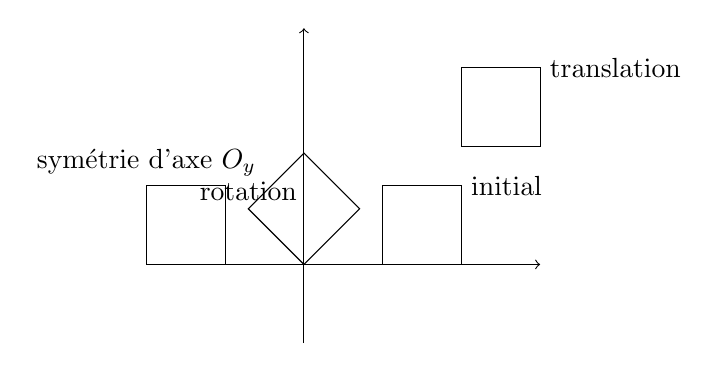
\begin{tikzpicture}
	\draw[->] (0, -1) -- (0, 3);
	\draw[->] (-2, 0) -- (3, 0);
	\draw[] (1, 0) rectangle (2, 1) node [right] {initial} ;
	\draw[] (2, 1.5) rectangle (3, 2.5) node [right] {translation};
	\draw[rotate=45] (1, 0) rectangle (0, 1) node [above, yshift=-0.5] {rotation};
	\draw[] (-1, 0) rectangle (-2, 1) node [above] {symétrie d'axe $O_y$};

\end{tikzpicture}
\end{wrapfigure}

Transformation du plan qui multiplie \ul{toutes} les longueurs par une même constante.

Prenons $cste = 1$ : La translations, la rotation et la symétries conviennent (ainsi que leurs composées).

Pour $cste \neq 1$ : l'homothétie de centre I et de rapport $\lambda$

\begin{wrapfigure}[6]{r}{0pt}
\begin{tikzpicture}
	\draw[->] (0, -1) -- (0, 3);
	\draw[->] (-2, 0) -- (3, 0);
	\draw[fill=black] (0, 0) circle (0.05) node [above] {$I$};
	\draw[thin] (-1, -1) -- (3, 3);
	\draw[] (1, 1) -- (1, 0) node [below] {$A$};
	\draw[] (2, 2) -- (2, 0) node [below] {$A'$};
	\draw[] (-0.5, -0.5) -- (-0.5, 0) node [above] {$A'$};

	\draw[fill=black] (1, 1) circle (0.05) node [above] {$B$};
	\draw[fill=black] (2, 2) circle (0.05) node [above] {$B'$};
	\draw[fill=black] (-0.5, -0.5) circle (0.05) node [above] {$B''$};
\end{tikzpicture}
\end{wrapfigure}


centre $(0, 0) = I$, $\lambda = 2$
\[\begin{array}{rcl}
A' &=& \text{ image de } A \\
B' &=& \text{ image de } B \\
\vec{IA'} &=& 2\vec{IA} \\
\vec{IB'} &=& 2\vec{IB}\end{array}\]

centre $(0, 0) = I, \lambda = -\frac{1}{2}$
\[\begin{array}{rcl}
\vec{IA''} &=& -\frac{1}{2}\vec{IA} \\
\vec{IB''} &=& -\frac{1}{2}\vec{IB}\end{array}\]

Les distances sont multipliées par $|\lambda|$

\paragraph{Définition} On appelle similitude directe une similitude qui préserve l'orientation. (c'est à dire on peut passer d'une triangle à son image en gardant le triangle dans le plan).

\paragraph{Theoreme} Une transformation T du plan est une similitude directe si et seulement si il existe $(a, b) \in \mathbb{C}, a \neq 0$ tels que ~\\
$\begin{array}{rcl}
T : \mathbb{C} &\rightarrow& \mathbb{C} \\
z &\mapsto& az + b\end{array}$

C'est à dire $\forall z \in \mathbb{C}, T(z) = az + b$

\paragraph{Remarque} Similitude directe

\begin{wrapfigure}[6]{r}{0pt}
\begin{tikzpicture}
	\draw[->] (0, -1.5) -- (0, 3);
	\draw[fill=black] (0, 0) circle (0.05) node [below left] {O};
	\draw[->] (-2, 0) -- (3, 0);
	\draw[fill=black, thick] (1, 1) circle (0.05) node [above, align=center] {$b (x, y) \in \mathbb{R}$ \\ $ \vec{OA}=(x, y)$};
	\node[below] at (1, 1) {$A$};
	\draw[fill=black] (1, -1.5) node [below right] {$B \to z_B$};
	\draw[fill=black] (2, -0.5) node [above right] {$B' \to z_B' = z_B + b$};
	\draw[thick] (1, -1.5) -- (2, -0.5);
\end{tikzpicture}
\end{wrapfigure}

\[T(z) = az + b, a \in \mathbb{C}^*, b \in \mathbb{C}\]

si $a=1$, $T(z) = z+b$. On a donc une translation de "vecteur" b

$b=(x+iy)$, translation de vecteur (x, y).

Si $b=0$, $T(z) =az, a \in \mathbb{C}^*$

C'est la composée d'une rotation d'angle arg(a) et d'une homothétie de rapport $|a|$ (et les deux de centre O)

cas général : $T(z) = az + b$

$z \rightarrow[translation]{} z+b \rightarrow[h+z]{} a(z+b) = az + ab$ Faux.

$z \rightarrow[h+z]{} az \rightarrow[translation]{} az + b = az + b$ Correct.

C'est faire l'homothétie et la rotation (dues à a) puis la translation (due à b)

Donc $T(z) =az + b$ est une similitude direct de :
\begin{itemize}
	\item de rapport $|a|$ 
	\item d'angle $arg(a)$
	\item de centre (si $a \neq 1$) $\frac{b}{1-a} \in \mathbb{C}$. Si $a=1$, il n'y a qu'une translation et une translation n'a aucun point fixe (et donc aucune rotation).
\end{itemize}

\paragraph{Remarque} Le centre est le seul point fixe de la transformation.
\[\begin{array}{rcl}
T{z_0} &=& z_0 \\
az + b &=&  z_0 \\
b &=& z_0 - az_0 = z_0(1-a) \\
z_0 = \frac{b}{1-a}
\end{array}\]

\paragraph{Exemple} $a=1, b = \frac{1}{2} + 3i$

Ceci est une translation de vecteur $(\frac{1}{2}, 3)$

\begin{wrapfigure}[6]{r}{0pt}
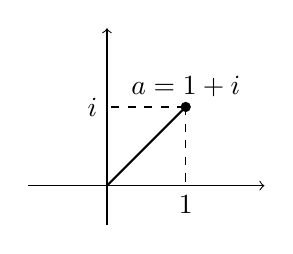
\begin{tikzpicture}
	\draw[->] (0, -0.5) -- (0, 2);
	\draw[->] (-1, 0) -- (2, 0);
	\draw[fill=black, thick] (0, 0) -- (1, 1) circle (0.05) node [above] {$a=1+i$};
	\draw[dashed] (1, 1) -- (0, 1) node [left] {$i$};
	\draw[dashed] (1, 1) -- (1, 0) node [below] {$1$};
\end{tikzpicture}
\end{wrapfigure}
$a = 1+i, b=0$

$|a| = \sqrt{1^2+1^2} = \sqrt{2}, arg(a) = \frac{\pi}{4}$

$T(z) = (1+i)z + (\frac{1}{2} + 3i)$ est

La composée de la rotation de centre O et d'angle $\frac{\pi}{4}$ et de l'homothétie de centre 0 et rapport $\sqrt{2}$. Puis de la translation de vecteur $\vec{\frac{1}{2}, 3}$

La similitude directe :

\begin{itemize}
\item d'angle $\frac{\pi}{4}$
\item de rapport $\sqrt{2}$
\item de centre $\frac{\frac{1}{2} + 3i}{1-(1+i)} = \frac{\frac{1}{2}+3i}{-i} = -3 -\frac{1}{2i} = -3 + \frac{i}{2}$
\end{itemize}

\paragraph{Remarque} IL suffit de connaître l'image de 2 points (distincts) pour déterminer la similitude.

Soit $s_1 \neq z_2$ dont connaît les images respectives $z_1' \neq z_2'$

\[\text{On a alors } \left\{\begin{array}{rcl}
z_1' &=& az_1 + b \\
z_2' &=& az_2 + b
\end{array}\right.\]

Donc $a = \frac{z_1' - z_2'}{z_1 - z_2}$ et donc $b= z_1' - \frac{z_1' - z_2'}{z_1-z_2}z_1$

\section{Formules trigonométriques}
\begin{wrapfigure}[6]{r}{0pt}
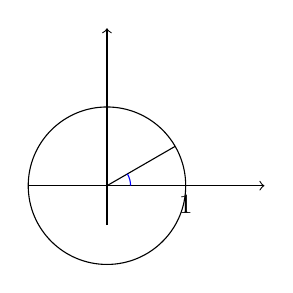
\begin{tikzpicture}
	\draw[->] (0, -0.5) -- (0, 2);
	\draw[->] (-1, 0) -- (2, 0);
	\draw[] (0, 0) circle (1);
	\draw[] (0, 0) -- (30:1);
	\draw[blue] (0.3, 0) arc (0:30:0.3);
	\draw[] (1, 0) node [below] {$1$};
\end{tikzpicture}
\end{wrapfigure}

Notation : $e^{i \theta} = \cos \theta + i \cdot \sin \theta$

\paragraph{Remarque} \[\begin{array}{rcl}
	\cos \theta &=& Re(e^{i\theta}) = \frac{e^{i\theta} + e^{-i\theta}}{2} \\
	\sin \theta = Im (e^{i\theta}) = \frac{e^{i \theta} 2 e^{-i\theta}}{2} \\
	z + \overline(z) = 2 Re(z)\end{array}\]

\paragraph{Propriété}
On a $e^{i\theta_i} \cdot e^{i\theta_2} = e^{i(\theta_1\cdot \theta_2)}$ pour tout $\theta_1, \theta \in \mathbb{R}$

\[\begin{array}{rcl}
		\text{Donc } \cos(\theta_1 + \theta_2) &=& Re(e^{i(\theta_1 + \theta_2)}) \\
											   &=& Re(e^{i\theta_1} \cdot e^{i\theta_2}) \\
											   &=& (\cos(\theta_1)+i\sin(\theta_1)) \cdot (\cos(\theta_2) + i \sin(\theta_2)) \\
											   &=& \cos(\theta_1) \cos(\theta_2) - \sin(\theta_1)\sin(\theta_2) + i(\sin(\theta_1)\cos(\theta_2) + \sin(\theta_2)\cos(\theta_1))\end{array}\]

		D'où $\cos(\theta_1 + \theta_2) = \cos(\theta_1)\cos(\theta_2) - \sin(\theta_1)\sin(\theta_2)$

		De même, $\sin(\theta_1+\theta_2) = \cos(\theta_1)\sin(\theta_2)+\cos(\theta_2)\sin(\theta_1)$

		\paragraph{Exercice} $\cos(\theta_1 - \theta_2); \sin(\theta_1 - \theta_2)$

		\paragraph{Proposition (formule de Moivre)}

		$\forall \theta \in \mathbb{R}, \forall n \in \mathbb{N} : e^{(i\theta)^n} = e^{in\theta}$

		C'est à dire $(\cos(\theta) + i \sin(\theta))^n = \cos(n\theta) + i \sin(n\theta)$

		\paragraph{Exercice}

		\[\begin{array}{rcl}
				\cos(3\theta) &=& Re(e^{i3\theta}) = Re((e^{i\theta})^3) \\
														 &=& Re((\cos\theta + i \sin\theta)^3) \\
											 &=& \cos^3 \theta - 3\cos \theta \sin^2 \theta\end{array}\]

				\paragraph{Exercice}
				À partir de $\cos(\theta_1\pm\theta_2)$ retrouver \[\cos\theta_1 \cdot \cos\theta_2 = \frac{\cos(\theta_1+\theta_2)+\cos(\theta_1-\theta_2)}{2}\]

				De même, retrouver, a partir de $\sin(\theta_1\pm\theta_2)$ retrouver \[\sin\theta_1 \cdot \sin\theta_2 = \frac{\cos(\theta_1-\theta_2)-\cos(\theta_1-\theta_2)}{2}\]
